\section{Result}
We have tested our method on a corpus provided by teacher. For detailed
escription of the corpus, please see former report.

All the tests are conducted serval times (depending on computation cost,
vary from 5 to 20) with random selected training and testing speakers.
The average over these tests are considered as the final
result.

\subsection{Effect Of Number Of Mixtures}
We examined our GMM compared to GMM from scikit-learn.
Test is conducted on 30-speaker corpus, 30 seconds training utterance
and 100 random sampled 5 seconds test utterance for each speaker.

\begin{figure}[!ht]
	\label{fig:mixture}
	\centering
	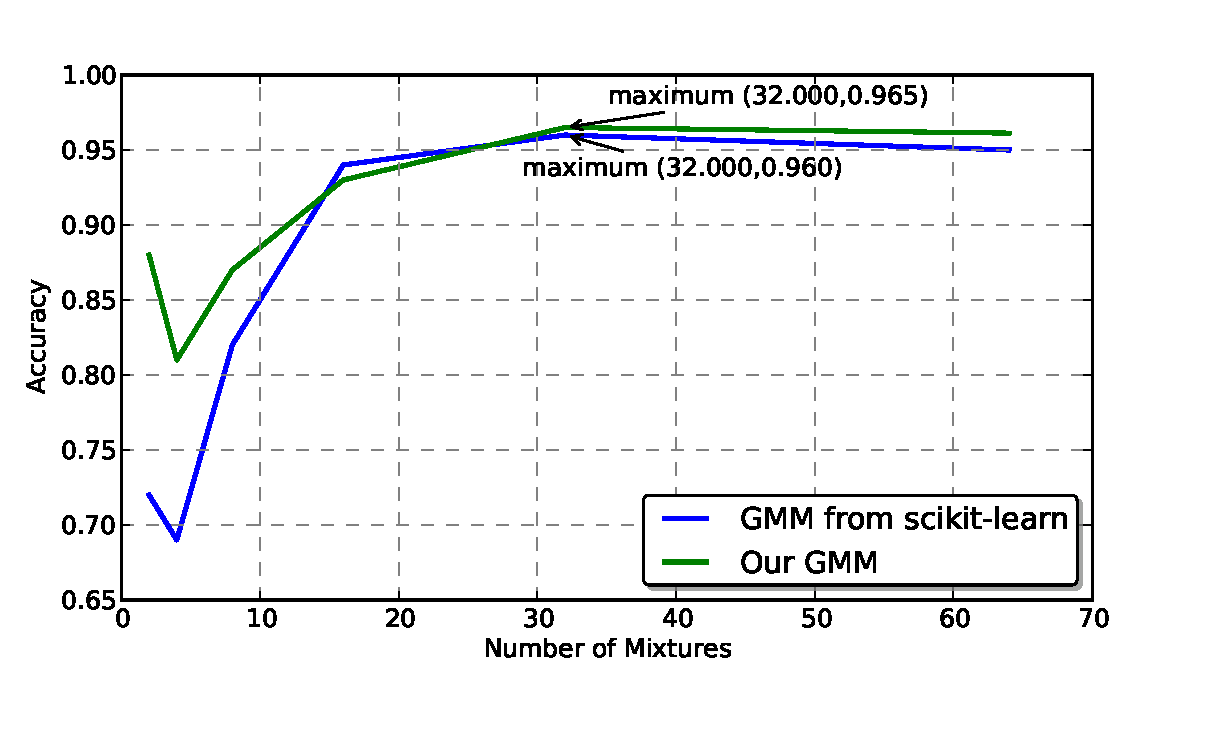
\includegraphics[width=\linewidth]{res/mixture-both.pdf}
	\caption{Accuracy curve on different number of mixtures}
\end{figure}

As \figref{mixture} illustrates, when number of mixtures is small,
our GMM outperforms scikit-learn version $10\%$, which indicates our
GMM models the distribution more accurate. The maximum accuracy
is when the number of mixtures is around 32, reaching $0.965$. As
the number of mixtures increase, the decrease in accuracy
may due to the overfitting to the training data.

\subsection{Effect Of Number Of Speakers Enrolled}
An apparent trade-off in speaker recognition task is the number of speakers
enrolled and the accuracy of recognizing a person. We've conduct experiments
examine the effect on number of speakers enrolled on the performance of the
system.

Here are the configurations of the test:
\begin{itemize}
	\item Number of mixtures is set to 32, the optimal number we found previously
	\item GMM from scikit-learn, compared to our GMM.
	\item 30s training utterance and 5s test utterance
	\item 100 sampled test utterance for each user
\end{itemize}

\begin{figure}[!ht]
	\label{fig:nspk_enrolled}
	\centering
	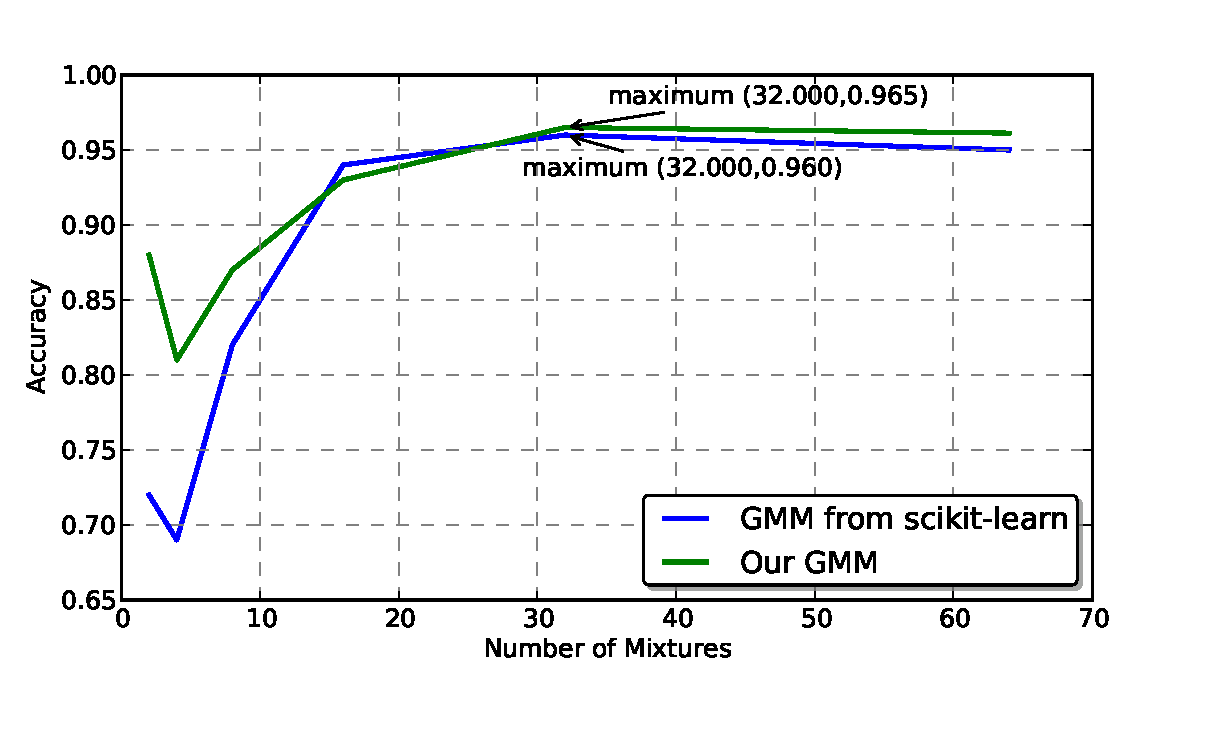
\includegraphics[width=\linewidth]{res/mixture-both.pdf}
	\caption{Accuracy curve on different number of speakers enrolled}
\end{figure}

Scrunitizing \figref{nspk_enrolled} we would see that, our GMM performs better than
scikit GMM in general. When number of speakers is small, due to the the random
selection, variance of the tests may high, as we can see the curve fluctuants.
When number of speakers increases, especially over 30, it is clear that the
accuracy of our GMM is constantly above scikit version. As the more speaker,
the more difficult the recognition task will be, this suggest that our
optimization on GMM takes effect.


